\section{16 bit addition}
\subsection{Aim}
To add two 16 bit numbers

\subsection{Code}
\begin{lstlisting}
ORG 0000H

; ROR1 forms 2000H
MOV R0, #20H
MOV R1, #00H

; R2R3 forms 3000H
MOV R2, #30H
MOV R3, #00H

; Addition of lower byte
MOV A, R1
ADD A, R3
MOV R5, A ; Lower byte of result stored in R5

; Addition of upper byte
MOV A, R0
ADDC A, R2
MOV R4, A ; Upper byte of result stored in R4

END
\end{lstlisting}

\subsection{Output}
\textbf{Input} 2000H (R0R1), 3000H (R2R3)\\
\textbf{Output} 5000H (R4R5)
\begin{center}
	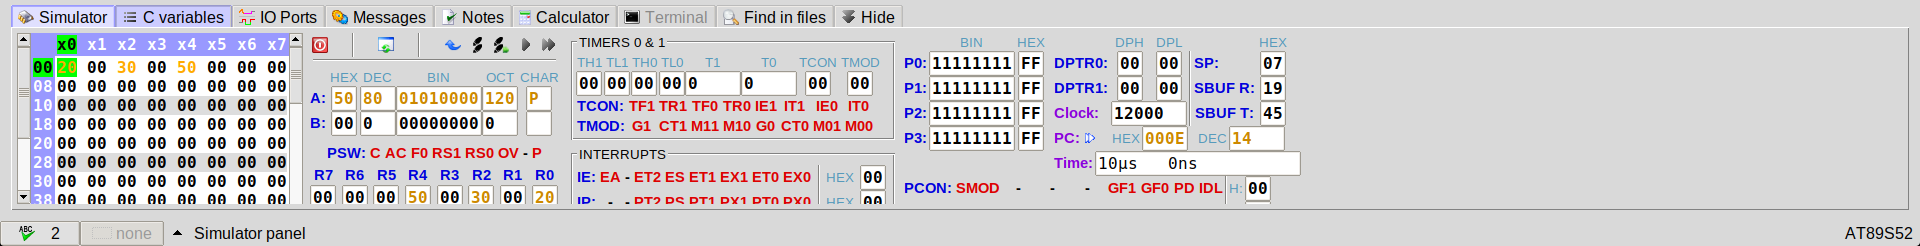
\includegraphics[width=\textwidth]{img/p21.png}
\end{center}

\subsection{Result}
Two 16 bit numbers were added in mcu8051ide

